\documentclass[
  journal=usp, %largetwo,
  manuscript=final-report,
  year=2023,
  volume=1,
]{cup-journal}

%\usepackage[backend=biber,citestyle=authoryear,bibstyle=numeric]{biblatex}
\usepackage{amsmath, bm}
\usepackage[nopatch]{microtype}
\usepackage{booktabs}
\usepackage{parskip}
%\usepackage{subfig}
%\usepackage{caption}
\usepackage{subcaption}
\usepackage{multicol}
\usepackage{hyperref}
%\usepackage{enumitem}
\usepackage{multirow}
\setlength{\parindent}{0pt} 

\SectionNumbersOn

\title{Study and evaluation of the unbinding kinetics of Mineralocorticoid receptor (MR) steroid agonist aldosterone, cortisol, and progesteron ligands using molecular modeling and simulations}

\author{Sebastian Aguilera Novoa}
\affiliation{Sao Carlos Institute of Physics, University of Sao Paulo, Brazil}
\alsoaffiliation{Natioanl University of Colombia, Physics Departament, Bogotá D.C, Colombia}
\email[S. A. N.]{saguileran@unal.edu}

\author{Alessandro S. Nascimento}
\alsoaffiliation{Sao Carlos Institute of Physics, University of Sao Paulo, Brazil}
%\email[A.S. Nascimento]{ asnascimento@ifsc.usp.br }

\addbibresource{example.bib}

\keywords{Amber, Molecular Dynamics, Monte Carlo, libela, ligand-protein, mineralocorticoid receptor, aldosterone, cortisol, progesterone, ligand binding.}

\begin{document}

\begin{abstract}
Insert abstract text here. \vspace{5cm}. asd
\end{abstract}


\section{1. Introduction}

The important role of the mineralocorticoid hormone aldosterone (MR/Aldo) in the cardiovascular system is well known, particularly its effects on the kidney which have been intensively studied. However, several investigations have demonstrated the importance of this hormone in the circulatory system. In fact, this hormone is related to several common diseases with high mortality and health care costs such as hypertension, stroke, heart failure, chronic kidney diseases, obesity, and diabetes disorders that appear when aldosterone is highly present. Since the main function of MR/Aldo is the regulation of renal sodium balance as well as biological effects, several researchers have reported its presence in organs such as kidney, heart, blood vessels, adipose tissue, brain, eyes, and skin \cite{book-MR_AS4, MR-as4_importance}, Figure \ref{MR_functions}.

\begin{figure}[htbp]
\centering
%\hspace*{-15pt}   
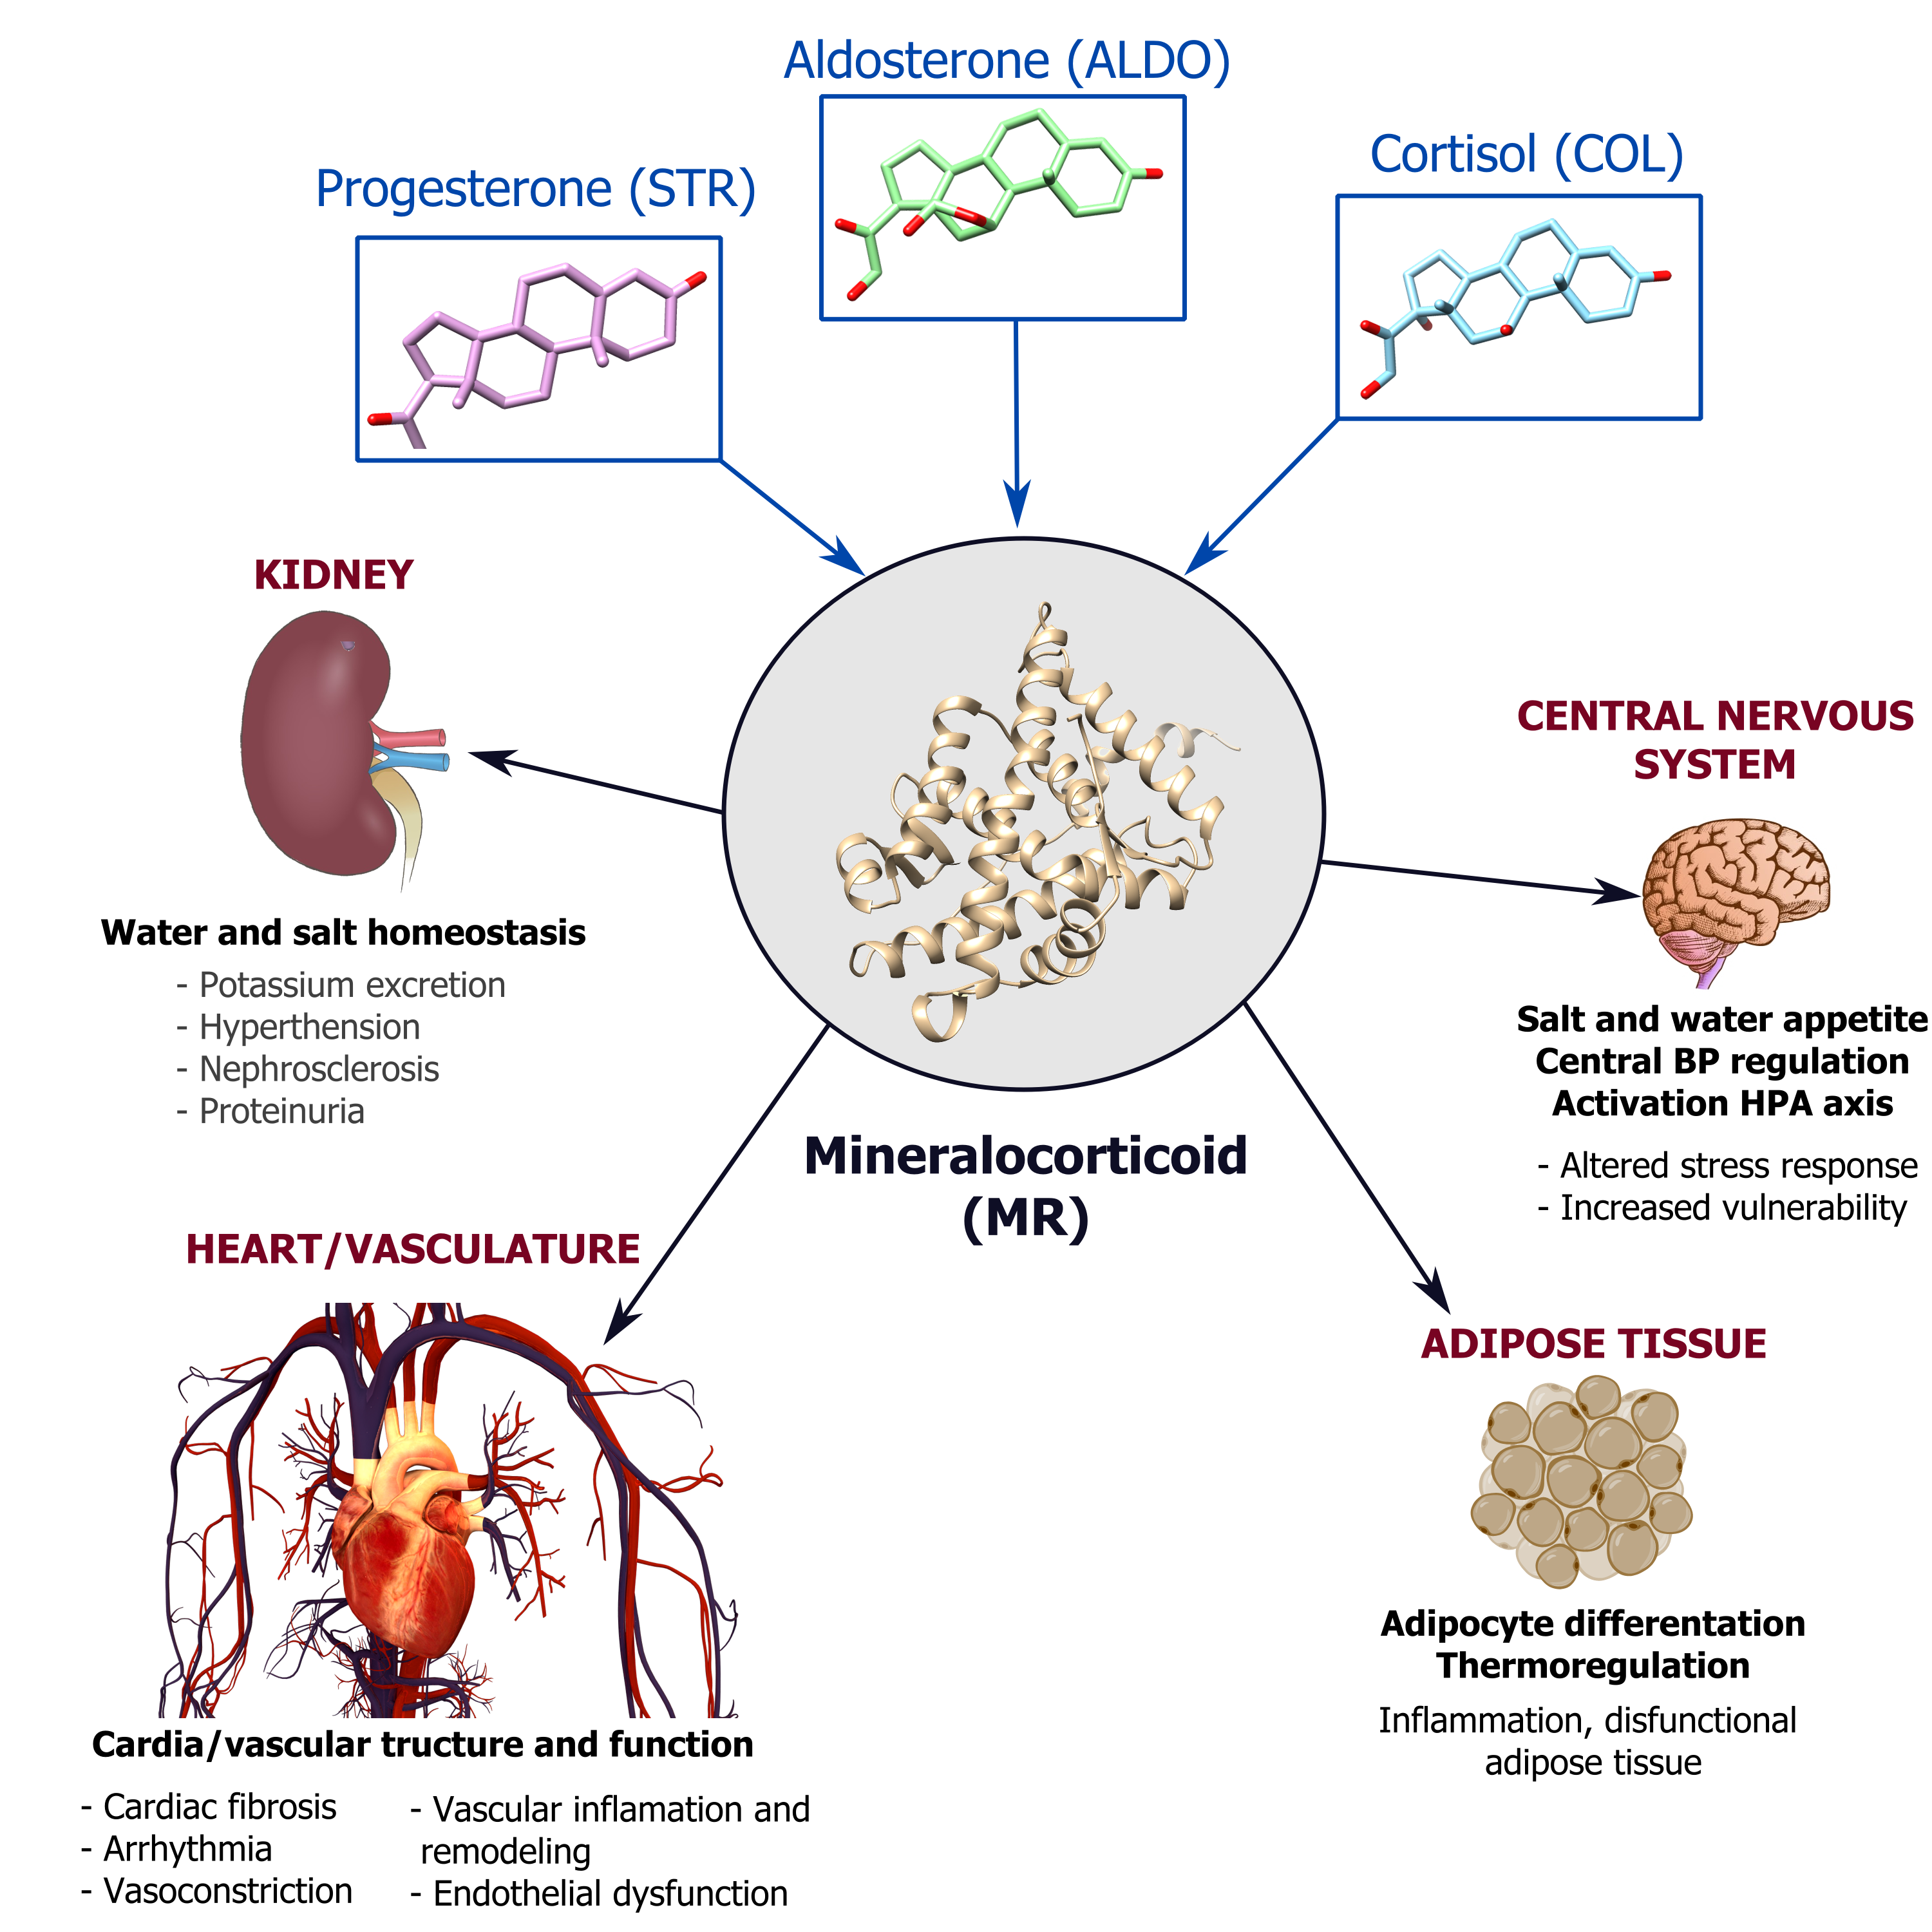
\includegraphics[scale=0.35]{Images/MR-AS4-COL.png}
\caption{Mineralocorticoid/aldosterone receptor impact on health. \textit{Image taken and adapted from} \cite{book-MR_AS4}.}
\label{MR_functions}
\end{figure}

The MR/aldo affinity has already been established, but a discovery at 1987 \cite{discovery}, the first studies with recombinant human MR (hMR), showed that hMR has strong binding affinities for several corticosteroids: aldosterone (aldo), cortisol (col), corticosterone, and 11-deoxycorticosterone; and for progesterone (str) \cite{book-MR_AS4}. Today is not well understood why MR is more sensitive to aldolsterone than to cortisol, this have been demonstrated by ex vivo experiments that also showed that the glucocorticoid cortisol hormone binds to the hMR with the same affinity as aldo, but is less efficient than aldo in stimulating the hMR transactivation \cite{HELLALLEVY20001250}.

Several studies on MR and its mutations have revealed that the substitution of leucine for serine at codon 810 (S810L) in hMR (MR$_{S810L}$) is responsible of early onset hypertension and pregnancy-related hypertension, which increase the risk of pre-eclampsia and early hypertension. Clinical studies in hypertensive patients and their families showed that all MR$_{S810L}$ carriers had developed hypertension before the age of 20 years, whereas those who do not present this mutant had normal blood pressure \cite{Severe, Activating_Mineralocorticoid}.

At present, the crystal structure of MR is known and has been obtained using different methods such as X-Ray Diffraction or Cryogenic Electron Microscopy (CryoEM); even recent articles on the glucocorticoid receptor (GR) suggested the asymmetric dimer form of MR \cite{dimer}. However, these methods only provide a static view of the protein's behavior and do not allow to adequately describe its dynamics: how does MR interact with a ligand in an un/binding process?. A trusted and explored approach to answer this question is molecular modeling. The enormous progress in computational resources has led us to developed robust and efficient methods to simulate proteins dynamics, such as Molecular Dynamics (MD) and Monte Carlo (MC) simulations, allowing researches to explore the dynamics of protein-ligand interactions and give strong explanations to their behavior and how they are interacting \cite{md_evidence} which is very useful for drug design, protein foldin or ligand binding.


%\textbf{talk about drug design, protein folding ligand binding}

%orphaz'n question

\section{2. State of Art}

% Selection of the best method to simulate the system, description of the simulation methods and how are we analyzing the date, since the MD simulations have a sense of time while the MC simulations does not, pyEMMA.

% Describe how LiGaMD and LiBELa works and the difference between them.

This section instroduces the necessary concepts and ideas for this work. This is followed by a brief description of the softwares currently used to simulate biomolecular dynamics. It is important to mention that computer simulations had a great evolution in the 1950s, where the development of computers made giant steps in numerical analysis giving a new perspective to the simulation of molecules. In fact, the last century gave rise to Molecular Dynamic (MD) and Monte Carlo (MC) simulations, in order to analyze the behavior of atoms and molecules, although MC simulations where previously proposed in the Manhattan Project, during World War II, by Stanislaw Ulam, John Von Neuman, and Nicholas Metropolis \cite{MD_history}, both have advanced enormously in recent years. 


\subsection{\textbf{2.1. Assisted Model Building with Energy Refinement (Amber)}}

Currently, one of the most widely used and tested package for setting up, performing, and analyzing MD simulations is Amber, a biomolecular simulation programs suite containing a set of molecular mechanical force fields for the simulation of biomolecules and a molecular simulation package programs with many scripts and tutorials.

Although Amber contains many tools, only few of them are used in this work to set up and perform MD simulations and generate the input files needed for molecular simulations:

\begin{itemize}
    \item \textbf{Antechamber (AC)}: classifies the tpyes of atom and bond, assings charges and estimates the force field parameters that may be missing in the gaff.dat file. These calculations are performed using quantum mechanics.
    \item  \textbf{General Amber Force Field (GAFF)}: defines the force field parameters in which a simple harmonic function is used for bonds and angles.
    \item \textbf{Gaussian program (g09 version)}: program used by AC to calculate electronic structure modelling: predict energies, molecular structures, and even more advanced calculations. It uses the fundamental laws of quantum mechanics.
    \item \textbf{LEaP}: stands link, edit, and parm, which are old amber function but in a single tool. It is the generic name given to the programs teLeap and xaLea. It is used to prepare the input files for AMBER molecular mechanics programs, it creates the \textit{prmtop} and \textit{inpcrd} files required for MD simulations.
    \item \textbf{cpptraj:} is the main amber trajectory analysis utility (written in C++) for performing out superpositions, coordinates extractions,  bond/angle/dihedral value calculations, atomic positional fluctuations, correlation functions, hydrogen bonds analysis, etc.
\end{itemize}

The greates advantage of this software is its good documentation and continues development, which improves year after year \cite{amber}.

\subsection{2.2. Molecular Dynamics (MD)}

The idea behind MD simulation is to solve Newton's second law of motion for several particles that can interact with each other, usually this method is called classical Molecular Dynamics (cMD) and is a deterministic approach. However, although the idea is simple many new techniques and models have been proposed to improve simulation performance, including code parallelization. The algorithms used in this work are:

\begin{itemize}
    \item \textbf{Simulated Annealing with NMR-Derived Energy Restraints (SANDER)}: is an Amber module that performs energy minimization, molecular dynamics, and NMR refinements. It provides direct support for various force fields for proteins and nucleic acids, and for various water models and other organic solvents. The basic force field involves potential energy of bonds, angles, dihedrals, and nonbinding atoms. \\
    
    \item \textbf{Particle Mesh Ewald Molecular Dynamics (PMEMD)}: is a version of SANDER  optimized for speed and parallel scaling. It is used to handle long-range electrostatic interactions such as van der Waals interactions that are estimated by a continuum model. \\
    
    \item \textbf{Locally-Enhanced Sampling (LES)}: is a simulation method in which several copies of a region, or a ligand, are created to smooth the interaction between the ligand and the protein.\\
    
    \item \textbf{Adaptive Steered Molecular Dynamics (ASMD)}: This method applies an external harmonic force on the physical system, ligand and protein, and drives a change in coordinates in a given time but with constant velocity. \\
    
    \item \textbf{Gaussian Accelerated Molecular Dynamics (GaMD):} is a robust computational method for simultaneous unconstrained enhanced sampling and free energy calculations of biomolecules. It works by adding a harmonic boost potential to smooth the system potential energy surface and reduce energy barriers. The boost potential follows Gaussian distribution \cite{gaussian_acelerated_basics}.\\
    
    \item \textbf{\textbf{Ligand Gaussian Accelerated Molecular Dynamics (LiGaMD)}}: is a recent GaMD-based algorithm that simulates ligand binding and unbinding, called ligand GaMD. It works by selectively boosting the ligand non-bonded interaction potential energy. In addition, it contains a second potential boost that can be applied to the remaining potential energy of the entire system in a dual-boost algorithm (\textbf{LiGaMD\_Dual}) to facilitate ligand binding \cite{ligamd_Miao}. \\

    The latest version of this algorithm is \textbf{LiGaMD2}, where the boost potential is applied to both the ligand and protein residues in the binding pocket to enhance the sampling of ligand binding and dissociation. It selects the ligand and the closest residues to apply the boost but the selection must be less than 500 atoms \cite{ligamd2}.
\end{itemize}

To run MD simulations it is useful to understand the two steps involved in a cMD simulation: equilibration and production. Because this work aims to reproduce the un/binding process of a ligand from a protein, the Molecular Mechanics Poisson-Boltzmann Surface Area (MM/PBSA) approach is used \cite{MMPBSA}, as it is an efficient and reliable free energy simulation method to simulate protein-ligand binding interactions. The steps involved in this algorithm are:

\begin{enumerate}
    \item Equilibrate the solvated complex:
    \begin{enumerate}%[leftmargin=.175pt]
        \item \textit{min.in}: minimize and optimize the distance between atoms to avoid overlaps, short distances result in numerical errors.
        \item \textit{heat.in}: gives velocities to the atoms to reach a temperature of 300 $K$.
        \item \textit{density.in}: equilibrates the density of the system by increasing the pressure at constant volume.
        \item \textit{equil.in}: relaxes the system at constant pressure and increasing volume keeping the velocity of teh atoms constant.\\
    All simulations use Langevin dynamics to control the temperature.    
    \end{enumerate}
    \item Production phase: \\
    \textit{prod.in}, lets the system evolve freely by solving the Newton's second law with an electrical potential defined by PMEMD (which is used for several models cMD, ASMD, or LiGaMD) or SANDLER (used by LES). It uses the same conditions as the \textit{equil.in} output, final phase of the equilibration process, to avoid an abrupt jump in the potential energy.
\end{enumerate}

For more information, please visit the Amber manual, tutorial \textit{7.4 Molecular Mechanics with a Poisson‐Boltzmann/Surface Area solvent: MM-PBSA} \cite{amber}.

%Molecular Mechanics Poisson-Boltzmann Surface Area (MM/PBSA)
%Amber PBSA is an analysis program for solvent-mediated energetics of biomolecules. A program for computing electrostatic and non-electrostatic continuum solvation free energies.

%pmemd A performance- and parallel-optimized dynamics engine implementing a subset of sander’s functionality

An alternative and new free option for users without cluster or GPUs is the \href{https://github.com/pablo-arantes/making-it-rain}{making-it-rain} project, which is based on \href{http://ambermd.org}{Amber} but using \href{https://colab.research.google.com/}{Google Colaboratory} as cloud computing \cite{making_it_rain}. 


%\textbf{how to analyze the results: is enough to create or use existing python scripts to count and detect un/binding process.}


\subsection{2.3. Monte Carlo (MC)}

Unlike MD simulations, MC method uses a stochastic approach to generate random samples following a Boltzmann distribution to obtain numerical results, using equilibrium statistical mechanics, since it was developed as an application of the Metropolis Monte Carlo simulation. Numerous papers have demonstrated the robustness of this method to simulate molecular dynamics. It employs a Markov chain procedure in order to determine a new state for a system from a previous one, the new state is selected such that it satisfies some statistical conditions, related to the energy of the new state.

Several softwares are available to perform MC simulations, but not all of them are designed to simulate ligand binding as is LiBELa.

\subsubsection*{\textbf{Ligand Binding Energy Landscape  (LiBELa)}}

LiBELa is a software that was developed as an alternative solution for docking in 2005 \cite{libela}, but has recently shown good results for ligand binding since it uses the MC method and Recursive MC (RMC) algorithm \cite{libela2}.

\textbf{how does it work?}



\subsection{2.3. \textbf{Python API for Emma's Markov Model Algorithms (PyEMMA)}}

This package has been developed for the estimation, validation and analysis of Markov models for molecular simulations. Since the MC simulations are random, whit no sense of time, it seems to be a good approach to analyze the data obtained.

The algorithms used for the analyze are:

\begin{itemize}
    %\item \textbf{Independent Components (ICs)}:
    
    \item  \textbf{Markov State Models (MSMs)}: are a class of powerful models for analyzing dynamical systems such as MD or even MC simulations. Its goal is to describe the system by means of a master equation such that the entire dynamics of the system can be described by just using MSM. \\
    
    Practically, the model consists in a \textit{transition probability matrix}, $n \times n$, in which the entire configuration space spanned by the system has been divided into $n$ states. By determining the states, it is possible to track the dynamical progress of a system (MC or MD simulation) by noting which state it occupies at time points separated by a lag time ($\tau$) which have to be Markovian, i. e., the system must be \textit{memoryless}: the probability that the system transitions to state $i$ given it is in state $j$, separed by an increment $\tau$, does not depend on where the system was before it entered state $j$ \cite{MSM}.\\

    
    \item  \textbf{Time-lagged Independent Component Analysis (TICA)}: 
    is a linear transformation method used to reduce the data dimensionality by mapping the usually high-dimensional input space into some lower-dimensional space that captures the relevant dynamics. Contrary to Principal Component Analysis (PCA), which finds the degrees of freedom of maximal variance, TICA finds the degrees of freedom of maximal autocorrelation at the given lagtime. 
    \textbf{missing to adapt} \\

    \item \textbf{Mean First Passage Times (MFPT)}:  \\
        
    \item \textbf{Cluster Algorithm k-means}:


    %\item  \textbf{Transition Path Theory (TPT) }:


    %\item  \textbf{hidden Markov state models (HMSMs)}:
    
\end{itemize}

PyEMMA analysis is typically used in the following steps:

\begin{enumerate}
    \item Data reading.
    \item Feature selection using a score function as VAMP.
    \item Coordinate transform and discretization, use TICA to reduce the data dimensionality.
    \item MSM estimation and validation.
    \item Data clustering analysis.
    \item Transition path theory.
\end{enumerate}

More information can be found at \href{http://emma-project.org/latest/}{PyEMMA - Emma’s Markov Model Algorithms's} homepage \cite{pyemma}.

\section{3. Methods}

The system of interest consists of a ligand bound to a protein within a binding pocket with strong interaction, as shown in Figure \ref{as4_scence}. Seven systems are studied in this work:

\begin{multicols}{2}
\begin{itemize}
    \item MR-Aldo
    \item MR-Col
    \item MR-Str 
    \item MR-Aldo$_{dimer}$
    \item MR$_{mut}$-Aldo
    \item MR$_{mut}$-Col
    \item MR$_{mut}$-Str
\end{itemize}
\end{multicols}

\vspace{-10pt}
where $_{mut}$ refers to the mutation of MR, MR$_{S810L}$, and $_{dimer}$ refers to the dimer system which consists of an asymmetric ligand-protein pair.

MD and MC simulation methods are used to study and evaluate the binding process of the above systems. Since MD simulations are longer than MC simulations, they are only tested on the MR-Aldo system but using different simulation parameters with the same software, LiGaMD, while MC simulations are tested for all seven systems.

%Describe the simulations, what parameters where used and why?

\begin{figure}[htbp]
\centering
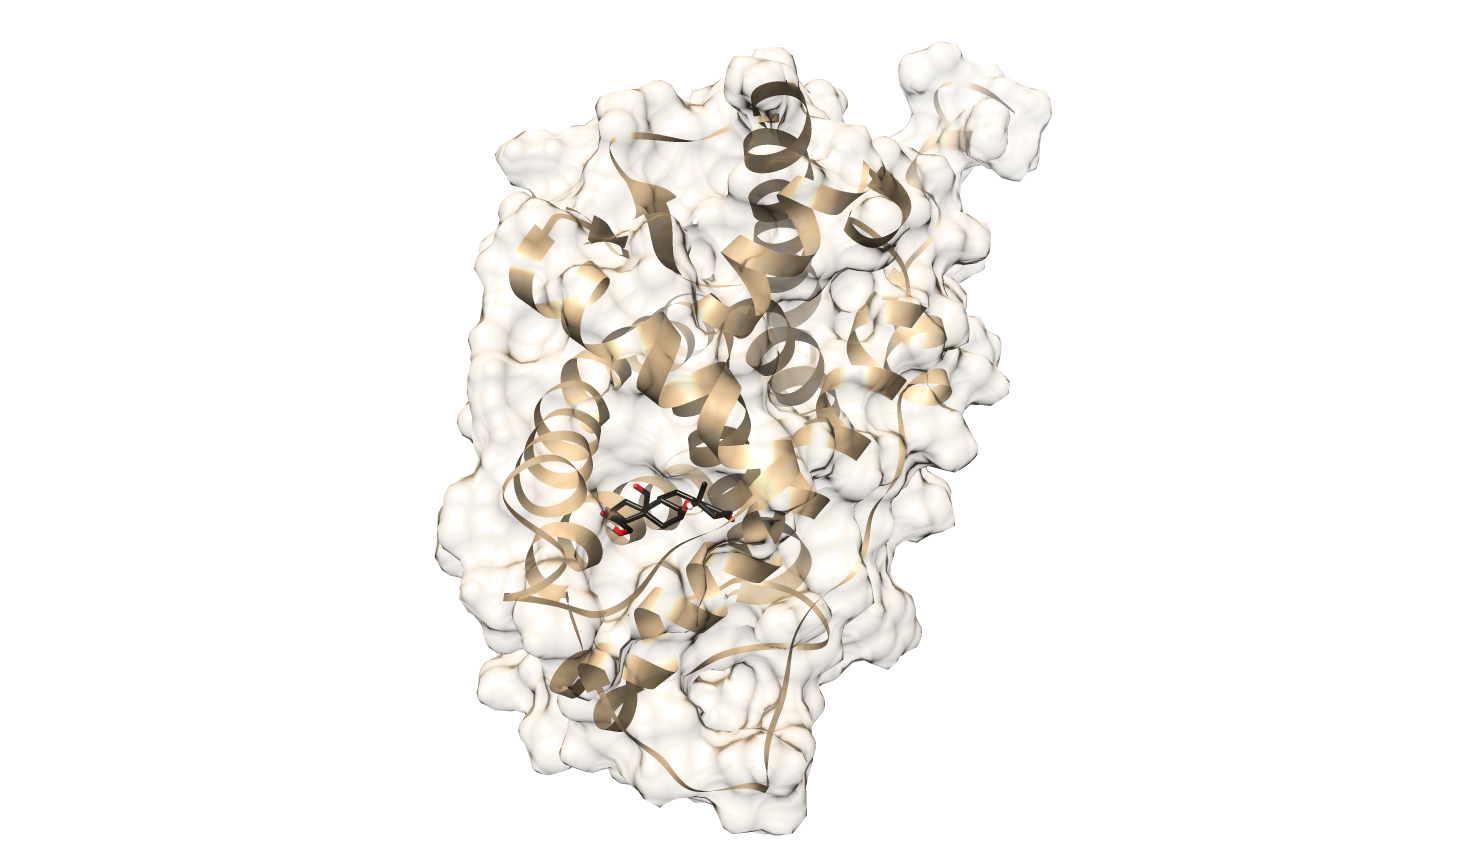
\includegraphics[width=0.9\linewidth]{Images/MR-AS4_escene.png}
\caption{Aldo ligand inside of the MR binding pocket.}
\label{as4_scence}
\end{figure}

The first step consists of generating the input files needed for the MD and MC simulation: \textit{PDBs}, \textit{mol2}, \textit{inpcr}, and \textit{prmtop} files. This was done with the amber tools described in the previous section following the steps below:

\begin{enumerate}
    \item Download and adapt the PDBs files of the proteins (MR and MR$_{S810L}$) and ligands (Aldo, Col, and Str) using \textit{Chimera}. 
    \item Calculate the atom charges and types with \textit{AC}.
    \item Define and compute the force field parameters with \textit{tleap} to generate the required input files to MD simulations: inpcrd and prmtop.
    \item Setup and execute MD simulation\footnote{for the MC simulations step 3 is omitted, since this simulation just required mol2 files}.
\end{enumerate}

The last step is to analyze the data from both simulations. This is done by computing energies with AmberEnergy++, to analyze ligand-protein interactions, and by analyzing the possible data states of MC simulations with PyEMMA, analyzing how frequently and "fast" the ligand escapes.
%What kind of simulation we ran and with which parameters. Why those values for MC and MD

\subsection{3.1. MD}
%: MR/Aldo, MR/Col, MR/Str,   MR$_{S810L}$/ Aldo, MR$_{S810L}$/Col, and MR$_{S810L}$/Str, 

The MD simulations were tested using the GaMD algorithm for all systems, while LiGaMD was only tested for the MR-Aldo system using different boost parameters for the simulations, as they can take several days. The simulation setups are presented in Table \ref{table_MD}. 

The simulations were set at a temperature of $300 \: K$ with a time step of $0.001 /: ps$. All simulations used the same parameters of $cut=8.0$, $ntb=2$, $ntp=1$, $taup=2.0$, $ntt=1$, $tautp=10.0$, and $barostat=2$; also the durations, in MD steps, of the involved process are: $ntcmd=7000000$, $nteb=27300000$, $ntave=140000$, $ntcmdprep=280000$, $ntebprep=2500000$. For more details visit the \href{http://miaolab.org/GaMD/manual.html}{GaMD manual} of the \href{http://miaolab.org/}{MIAO Lab}.


\begin{table}[htbp]
\begin{threeparttable}
\caption{Parameters used in the MD simulations for the MR/Aldo system}
\label{table_MD}
\begin{tabular}{|ccccc|}
\toprule
\headrow \textbf{Boost} & \bm{$\sigma_P$} & \bm{$\sigma_D$} & \textbf{Long [MD steps]}  &  \textbf{LiGaMD version}\\\midrule
single & 5 & NA  & 100M & 1 \\ \midrule
single & 6 & NA & 100M & 1 \\ \midrule
double & 4 & 6 & 100M & 1 \\ \midrule
double & 6 & 6 & 100M & 1 \\ \midrule
double & 6 & 8 & 100M & 1 \\ \midrule
double & 8 & 6 & 100M & 1 \\ \midrule
double & 10 & 8 & 100M & 1 \\ \midrule
double & 12 & 10 & 100M & 1 \\ \midrule
double & 6 & 6 & 100M & 2 \\ \midrule
double & 6 & 6 & 300M & 2 \\ \midrule
double & 6 & 10 & 100M & 2 \\
\bottomrule
\end{tabular}
\begin{tablenotes}[hang]
\item[] NA: Not Apply. M: million, equivalent to $1$ ns because the step is $0.001$ ps. All simulations are at a temperature of 300 K.
\end{tablenotes}
\end{threeparttable}
\end{table}

The LES algorithm was also tested for the MR-Aldo system with and without solvent, but these simulations present poor performance or several errors, so no further tests were done. 

In addition, the ASMD algorithm was also tested for all single systems (not dimer) using the previous GaMD output files as input since this algorithm requires the final distance of the Center of Mass (CM) of the ligand to the CM of the protein. Although the CM is easy to calculate using \textit{cpptraj} for both ligand and protein, the CM of the ligand is defined as the closest molecule to the CM making it easier to set up.


\subsection{3.2. MC}

The MC simulations were implemented with LiBELa. The first step was to explore the impact of the MC temperature in the MR-Aldo system, looking at what temperatures the system exhibited un/binding process and how the energy varied as a function of RMSD, and how long the simulations  should last. Then, once the temperatures of interest were selected ($5000 \:K$ and $7000 \:K$), the other systems were set up and ran at the selected temperatures with the same total number of LiBELa steps, Table \ref{table_MC}. 

\begin{table}[htbp]
\begin{threeparttable}
\caption{Parameters used in the MC simulations}
\label{table_MC}
\begin{tabular}{|ccc|}
\toprule
\headrow \textbf{Ligand} & \textbf{Temperatures [\bm{$K$}]} & \textbf{Length [LiBELa steps]} \\
\midrule
Aldo & 300, 600, 1200, 2400, 4800, 5000, & 30M, 50M,\\ 
     & 7000, 9600, 10000, 15000, 20000  & 100M \\  \midrule
Col & 5000, 7000 & 100M\\\midrule
Str & 5000, 7000 & 100M \\ \midrule
Aldo$_{mut}$ & 5000, 7000 & 100M\\ \midrule
Col$_{mut}$ & 5000, 7000 & 100M\\ \midrule
Str$_{mut}$ & 5000, 7000 & 100M\\ \midrule
Aldo$_{dimer}$ & 5000, 7000, 10000, 15000 & 100M\\ 
\bottomrule
\end{tabular}
\begin{tablenotes}[hang]
\item[] The sub-index $_{mut}$ refers to the mutation MR$_{mut}$ (MR$_{S810L}$), while $_{dimer}$ refers to the dimer system, an antisymmetric pair of ligand-protein.
\end{tablenotes}
\end{threeparttable}
\end{table}

All simulations use the following LiBELa parameters: search box = grid box= 30.0 \AA $\times$ 30.0 \AA $\times$ 30.0 \AA, scoring function = 0, ligand energymodel = GAFF, atomic model ff = AMBER, cushion = 0.25, max atomisplacement = 0.01 \AA, rotation step = 1.25 \AA, and torsion step = 1.25 \AA. The  most important parameter is the \textbf{cushion}, which was selected so that the acceptance rate of the MC simulation for the protein is between 0.3-0.5. 

\section{4. Results and Discussion}

%Select images of interest and explain them

\subsection{4.1. MD}

%Talk about the energy vs time plots that shows what protein atoms interact strongly with the ligand, this can help to understand how the ligand can scape from the pocket


%for the seven systems at a temperature of 300 K. The simulation involves an equilibration (min, heat, density, and equil) process, to obtain an equilibrated system, and a production (prod) process to obtain an ensemble of snapshots where the system is evolving in time \cite{amber}. 

The MD simulations showed that with LiGaMD it is possible to characterize the protein-ligand thermodynamics and kinetics. In fact, using the output files of the simulations the total energies of interaction, due to the van der Waals and Coulomb potentials, were computed between the ligand and the protein, the environment, and the closest residues: GLN51, ASN45, ARG92, SER118, HH22, THR222, and SER85, revealing that the ligand interacts mainly with residues GLN51, ASN45, and ARG92, while the others residues do not involve relevant changes in the total energy, as shown in Figure \ref{MD_energies}.

Although several MD simulations of the MR-Aldo system were set up and execute with two algorithms, LiGaMD 1 and 2, none of the simulations reproduce un/binding events. This suggests that the binding pocket is very strong and that these algorithms are not sufficient, even using high values of boost parameters in dual boost, to emulate ligand escape even though LiGaMD2 has demonstrated a strong ability to reproduce the un/binding process. 


%It happens because the applied boost is not enough to let the ligand escape from the pocket that it is in, \textit{ligand binding pocket}	

%The last version of this software, LiGaMD2, illustrate how to use it for ligand binding simulations. The biggest difference with the first version is that for the residues and its surroundings, protein residues, a selective boost potential is applied to improve sampling of ligand binding and dissociation. Since the simulations take several days, in the best case a few, the simulations is only tested in the MR/Aldo system since it present the strongest interaction.

\subsection{4.2. MC}

%Talk about how the energy was selected, how the un/binding events were counted and what does it means. Additional talk about how the data analyze

% 


The plot of energy as a function of Root Mean Square Deviation (RMSD), Figure \ref{MC_RMSD_energy}, shows how at low temperatures, below 4800 $K$, the ligand cannot escape, even when the energy (temperature) increased the RMSD of the ligand did not increase and did not cross the RMSD threshold (11 \AA); while for high temperatures, above 5000 $K$, many samples exhibit un/binding events visualized as an increase in the RMSD of the ligand. 

To analyze the ligand behavior, the RMSD of the ligand is plotted as a function of LiBELa steps, Figure \ref{MC_RMSD_steps}, where the un/binding events are readily apparent and marked with an X. These events were counted and the probabilities of occurrence, rate of un/binding events over the total number of samples, were calculated. The results are presented in Table \ref{MC_table_results}.

However, although this calculation gives an idea of the magnitude of events, it is not accurate because the implemented algorithm is very simple. Therefore, an MSM and TICA analysis is required, which are implemented in the PyEMMA package. 

The analysis of the six individual systems\footnote{without dimer system} using PyEMMA shows the presence of at least two macrostates in all cases: \textbf{bound} and \textbf{unbound} states, as can be seen in any plot in Figure \ref{fig:all-states}. In some cases, each macrostate was divided into two microstates: for the \textit{bound} state an \textbf{in pocket} and \textbf{flipped} states were found; while for the \textit{unbound} state two microstates were found, i.e., the two different unbinding pathways that the ligand can have, however, these microstates were difficult to define and it was not possible to obtain them in all cases, for all the systems. 

Macrostates were calculated for all systems obtaining two different unbinding pathways for the MR wild protein, whereas when the mutation, MR$_{S810L}$, is present only one unbinding pathway is observed for Col and Str, as can be seen by comparing the Figures \ref{MC_states_MR-as4} and \ref{MC_states_MR-as4_mut} for example. This suggests that the mutation eliminates a pathway, i.e., the changed residue  modifies the interaction with the neighboring ligand and blocks the ligand in some way.

To analyze the ease and frequency with which the system changes from one state to another, mainly from the bound state to others and vice-versa, TICA and MFPT analysis functions were used with a \textit{lagtime} of 10, the results are present in Table \ref{MFPT_bound} which indicates that the mutation increases the number of steps required to the ligand escape, e.i., the ligand unbinding is "faster" in the wild type whereas the mutation is present the unbinding is slower.

\begin{table}[htb]
\begin{threeparttable}
\caption{MFPT analysis of the bound state with the others.}
\label{MFPT_bound}
\begin{tabular}{|c|c|c|}
\toprule
\headrow \textbf{Ligand} & \textbf{MFPT bound $\bm{\to}$ other} & \textbf{MFPT other $\bm{\to}$ bound} \\\midrule
Aldo            & 511.8 ±   8.3 & 34229.1 ± 5028.2 \\ %\hline
Col             & 512.9 ±   8.9 & 163482.9 ± 31149.2 \\% \hline
Str             & 267.7 ±   3.3 & 57136.8 ± 8330.1 \\ \hline
Aldo$_{mut}$    & 797.7 ±  16.4 & 38229.3 ± 5514.4 \\ 
Col$_{mut}$     & 968.2 ±  21.5 & 53617.9 ± 5090.8 \\ %\hline
Str$_{mut}$     & 446.2 ±   5.5 & 9677.0 ± 1095.6 \\ %\hline
\bottomrule
\end{tabular}
\begin{tablenotes}[hang]
\item[] The units of both columns are LiBELa steps. The bound state is the number 2 in all the systems, as can be seen in Figure \ref{fig:all-states}.
\end{tablenotes}
\end{threeparttable}
\end{table}




%Comparing these two tables is possible to see that for the mutation the numbers are lower than for the wild type protein suggesting that the mutation makes easier to escape the lingad?


%For low temperatures the simulation do not present un/binding events but for high temperature, over than 5000 $K$, the ligand starts to un/binding easily. To analyze the un/binding events a python code was wrote, it counts the number of times where the RMSD cross a threshold of 11 \AA, results are present in Table \ref{table_MC_binding_couts}.

%Figures \ref{MC_RMSD_energ=y} and \ref{MC_RMSD_steps}
%Table \ref{MC_table_results}
%Figures \ref{MC_states_MR-as4} and \ref{MC_states_MR-as4_mut} 

%\subsection{Mean First Passage Times (MFPT)}

% % ----------------- MR-aldo -----------------
% \begin{table}[htbp]
% \begin{threeparttable}
% \caption{MFPT for the MR-Aldo system}
% \label{table_MC_MFPT_as4}
% \begin{tabular}{|c|ccc|}
% \toprule
% \headrow & \textbf{1} & \textbf{2} & \textbf{3} \\ \midrule
% \textbf{1} & 0.0	     & 1363.7	 & 21452.1 \\
% \textbf{2} & 1417.9	 & 0.0	     & 21493.2 \\
% \textbf{3} & 41508.3	 & 41498.5		 & 0.0 \\ 
% \bottomrule
% \end{tabular}
% \end{threeparttable}
% \end{table}

% \begin{table}[htbp]
% \begin{threeparttable}
% \caption{MFPT for the MR-Aldo$_{mut}$ system}
% \label{table_MC_MFPT_as4_mut}
% \begin{tabular}{|c|ccc|}
% \toprule
% \headrow & \textbf{1} & \textbf{2} & \textbf{3} \\\midrule
% \textbf{1} & 0.0	 & 2491.7	 & 12451.0 \\
% \textbf{2} & 3296.1	 & 0.0	     & 12442.1 \\
% \textbf{3} & 38690.2 & 37897.6	 & 0.0 \\ 
% \bottomrule
% \end{tabular}
% \end{threeparttable}
% \end{table}


% % ----------------- MR-col -----------------
% \begin{table}[htbp]
% \begin{threeparttable}
% \caption{MFPT for the MR-Col system}
% \label{table_MC_MFPT_col}
% \begin{tabular}{|c|ccc|}
% \toprule
% \headrow & \textbf{1} & \textbf{2} & \textbf{3} \\ \midrule
% \textbf{1} & 0.0	     & 7327.7	 & 13156.0 \\
% \textbf{2} & 7063.0	 & 0.0	     & 13190.8 \\
% \textbf{3} & 164213.3 & 164602.0	 & 0.0 \\ 
% \bottomrule
% \end{tabular}
% \end{threeparttable}
% \end{table}

% \begin{table}[htbp]
% \begin{threeparttable}
% \caption{MFPT for the MR-Col$_{mut}$ system}
% \label{table_MC_MFPT_col_mut}
% \begin{tabular}{|c|ccc|}
% \toprule
% \headrow & \textbf{1} & \textbf{2} & \textbf{3} \\\midrule
% \textbf{1} & 0.0	 & 3863.0	 & 26917.8 \\
% \textbf{2} & 3160.2	 & 0.0	     & 27127.8 \\
% \textbf{3} & 76355.4	 & 77321.5	 & 0.0 \\ 
% \bottomrule
% \end{tabular}
% \end{threeparttable}
% \end{table}


% % ----------------- MR-str -----------------
% \begin{table}[htb]
% \begin{threeparttable}
% \caption{MFPT for the MR-Str system}
% \label{table_MC_MFPT_str}
% \begin{tabular}{|c|ccc|}
% \toprule
% \headrow & \textbf{1} & \textbf{2} & \textbf{3} \\ \midrule
% \textbf{1} & 0.0	     & 4054.8	& 18666.2 \\
% \textbf{2} & 319479.2	 & 0.0	     & 14627.1 \\
% \textbf{3} & 367610.3	& 48103.3	 & 0.0 \\ 
% \bottomrule
% \end{tabular}
% \end{threeparttable}
% \end{table}

% \begin{table}[htb]
% \begin{threeparttable}
% \caption{MFPT for the MR-Str$_{mut}$ system}
% \label{table_MC_MFPT_str_mut}
% \begin{tabular}{|c|ccc|}
% \toprule
% \headrow & \textbf{1} & \textbf{2} & \textbf{3} \\\midrule
% \textbf{1} & 0.0	 & 692.0	& 19697.6 \\
% \textbf{2} & 778.6	& 0.0	& 19704.5 \\
% \textbf{3} & 15060.7	& 14982.3		 & 0.0 \\ 
% \bottomrule
% \end{tabular}
% \end{threeparttable}
% \end{table}










%\begin{figure}[htbp]
%\centering
%
\includegraphics[width=0.9\linewidth]{Images/example-image.pdf}
%\caption{Example states found for the MR-Aldo system using PyEMMA}
%\label{MC_states_examples}
%\end{figure}


\subsection{4.3. ASMD}

Missing results and analysis






\section{5. Conclusion}

\begin{itemize}

\item Although LiGaMD-1/2 has demonstrated a tremendous ability to reproduce un/binding process for the systems of interest, MR-MR${mut}$/Aldo-Col-Str, the algorithm does not reproduce un/binding events, no matter how long the simulation is or how high the boost parameters are. This is because the ligand is inside a pocket with a high barrier, the electrical potential between the ligand and protein is very strong and the boost is not enough. 

\item LiBELa is able to reproduce un/binding in MR-MR${mut}$/ Aldo-Col-Str systems, even when it simulates only the dynamics of the ligand and considers the protein as fixed. This shows how powerful the software is even in systems where the binding pocket is buried, which makes dissociation difficult.

\item PyEMMA package shows a great solution for analyzing MC simulation since using it in the generated data it is possible to find different states of the system: inside the pocket (\textbf{bound} state), inside the pocket but \textbf{flipped}, and an \textbf{unbound} state (where the ligand is outside the protein); the software even shows the different existing pathways for the ligand to escape by classify them into two different microstates. 

\item The MC simulations reveal that the mutation of MR (MR$_{S810L}$) makes the unbinding longer, i.e., for the ligand to escape more LiBELa steps are required. The easiest escaping ligand is the Str, which can be explained because it does not have the same oxygens molecules as the others and make the interaction with the protein weaker; while Col and Aldo need a similar number of LiBELa steps to escape from the MR protein as can be seen in Table \ref{MFPT_bound}.    

%Further analysis is applied to quantify how easy, or frequently, it is for the ligand to escape in terms of frames, as MC simulations have not sense of time.

\end{itemize}


% \begin{table}[hbt!]
% \begin{threeparttable}
% \caption{An Example of a Table}
% \label{table_example}
% \begin{tabular}{llll}
% \toprule
% \headrow Column head 1 & Column head 2  & Column head 3 & Column head 4\\
% \midrule
% One\tnote{a} & Two&three three &four\\ 
% \midrule
% Three & Four&three three\tnote{b} &four\\
% \bottomrule
% \end{tabular}
% \begin{tablenotes}[hang]
% \item[]Table note
% \item[a]First note
% \item[b]Another table note
% \end{tablenotes}
% \end{threeparttable}
% \end{table}


%\twocolumn{


% \begin{acknowledgement}
% Insert the Acknowledgment text here.
% \end{acknowledgement}

\paragraph{Funding Statement}

This research was supported by grants from the \href{https://www.ifsc.usp.br/crint/call-for-internships/}{Jhoti-Cortés-Salazar scholarship}, Institute of Physics of São Carlos (IPSC), University of São Paulo (USP).

% \paragraph{Competing Interests}

% A statement about any financial, professional, contractual or personal relationships or situations that could be perceived to impact the presentation of the work --- or `None' if none exist.

\paragraph{Data Availability Statement}

%A statement about how to access data, code, and other materials allowing users to understand, verify and replicate findings --- e.g. 
Replication data and code can be found on GitHub at
\href{https://github.com/saguileran/MD-SCPI/}{www.github.com/saguileran/MD-SCPI/}, or for a more detailed description \href{https://saguileran.github.io/MD-SCPI/}{www.saguileran.github.io/MD-SCPI}.
%}


%\endnote in some journals will behave like \footnote; and \printendnotes will not output anything. 

\onecolumn{
\appendix

\section{\centering Appendix}
\vspace{10pt}

\begin{table}[htbp]
\begin{threeparttable}
\caption{Un/binding MC events counted for all the systems using a simple python script \href{https://github.com/saguileran/MD-SCPI/blob/main/NoteBooks/Plots_MC.ipynb}{Plots\_MC.ipynb}.}
\label{MC_table_results}
\begin{tabular}{|cccccc|}
\toprule
\headrow \textbf{Ligand} & \textbf{Temperature [$\bm{K}$]} & \textbf{Unbinding Events} & \textbf{Binding Events} & \textbf{Unbiding$\bm{_{prob}}$ [\%]} & \textbf{Biding$\bm{_{prob}}$ [\%]}\\
\midrule
AS4 	    	& 5000K 	& 0 	& 1 	& 0.00 		& 1.96 \\
AS4 	    	& 7000K 	& 2 	& 20 	& 3.92 		& 39.22 \\ \midrule
COL 	    	& 5000K 	& 0 	& 0 	& 0.00 		& 0.00 \\
COL 	    	& 7000K 	& 0 	& 28 	& 0.00 		& 54.90 \\ \midrule
STR 	    	& 5000K 	& 0 	& 0 	& 0.00 		& 0.00 \\
STR 	    	& 7000K 	& 4 	& 30 	& 7.84 		& 58.82 \\ \midrule
AS4$_{mut}$ 	& 5000K 	& 0 	& 3 	& 0.00 		& 5.88 \\
AS4$_{mut}$ 	& 7000K 	& 2 	& 30 	& 3.92 		& 58.82 \\ \midrule
COL$_{mut}$ 	& 5000K 	& 0 	& 3 	& 0.00 		& 5.88 \\
COL$_{mut}$ 	& 7000K 	& 0 	& 14 	& 0.00 		& 27.45 \\ \midrule
STR$_{mut}$ 	& 5000K 	& 0 	& 0 	& 0.00 		& 0.00 \\
STR$_{mut}$ 	& 7000K 	& 5 	& 19 	& 11.76 	& 37.25 \\ \midrule
AS4$_{diemr}$ 	& 5000K 	& 6 	& 19 	& 11.76 	& 37.25 \\
AS4$_{diemr}$ 	& 7000K 	& 92 	& 124 	& 180.39 	& 243.14 \\
\bottomrule
\end{tabular}
\begin{tablenotes}[hang]
\item[] All simulations have 51 samples. The sub-index $_{mut}$ and $_{dimer}$ refers to the system with the MR mutation (MR$_{S810L}$) and the dimer system, double ligand and protein where just one ligand is moving.
\end{tablenotes}
\end{threeparttable}
\end{table}


\vspace{80pt}

\begin{figure*}
\vspace{-60pt}
\centering
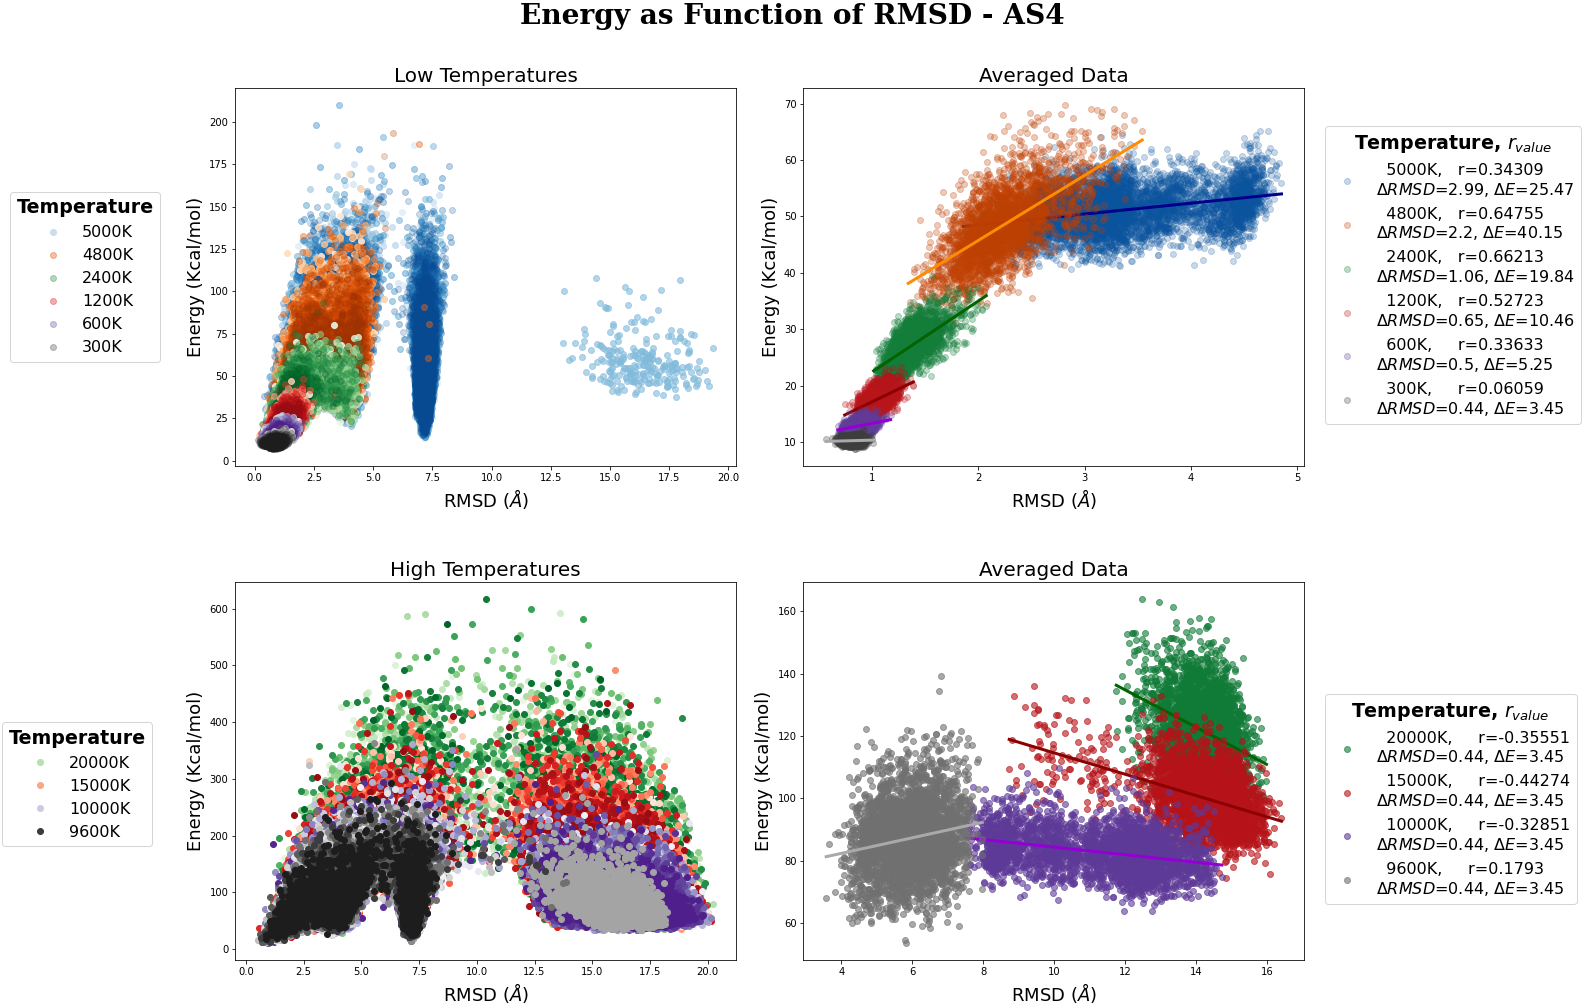
\includegraphics[width=0.9\linewidth]{Images/MC_energies.png}
\caption{RMSD as function of energy for the MR-Aldo system using MC simulation.}
\label{MC_RMSD_energy}
\end{figure*}


\begin{figure}[hbt!]

\begin{subfigure}{.45\linewidth}
  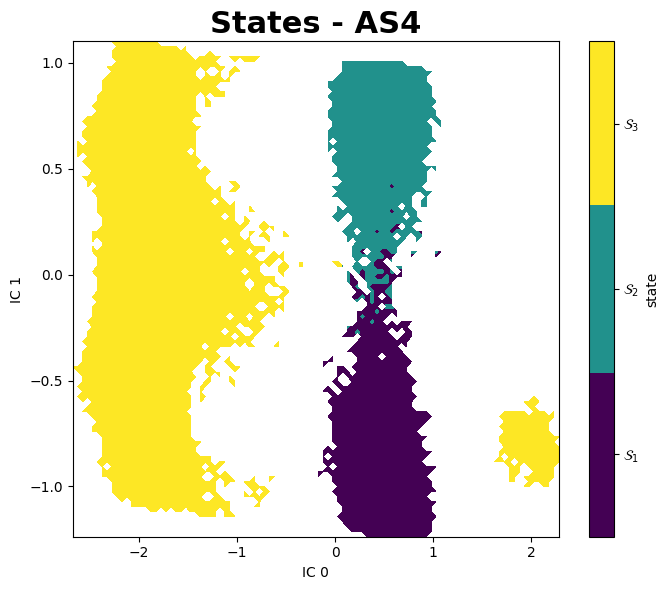
\includegraphics[width=\linewidth]{Images/States_AS4_7000K.png}
  \caption{MR-Aldo}
  \label{MC_states_MR-as4}
\end{subfigure}\hfill % <-- "\hfill"
\begin{subfigure}{.45\linewidth}
  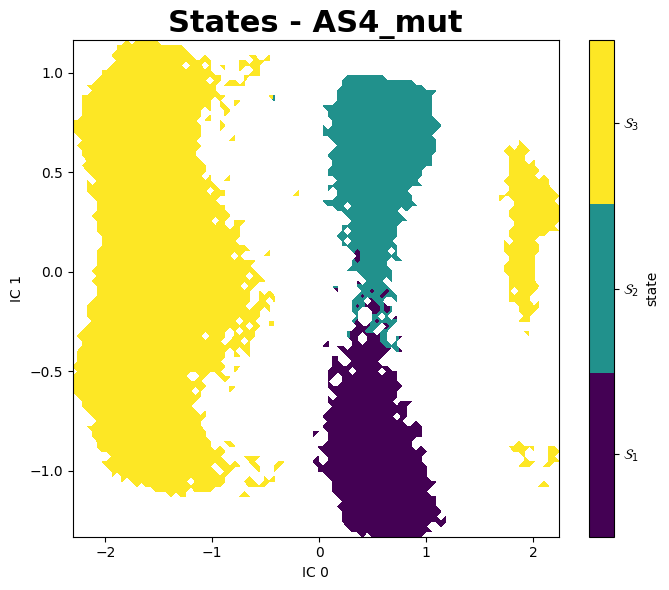
\includegraphics[width=\linewidth]{Images/States_AS4_mut_7000K.png}
  \caption{MR$_{mut}$-Aldo}
  \label{MC_states_MR-as4_mut}
\end{subfigure}

\medskip % create some *vertical* separation between the graphs
\begin{subfigure}{.45\linewidth}
  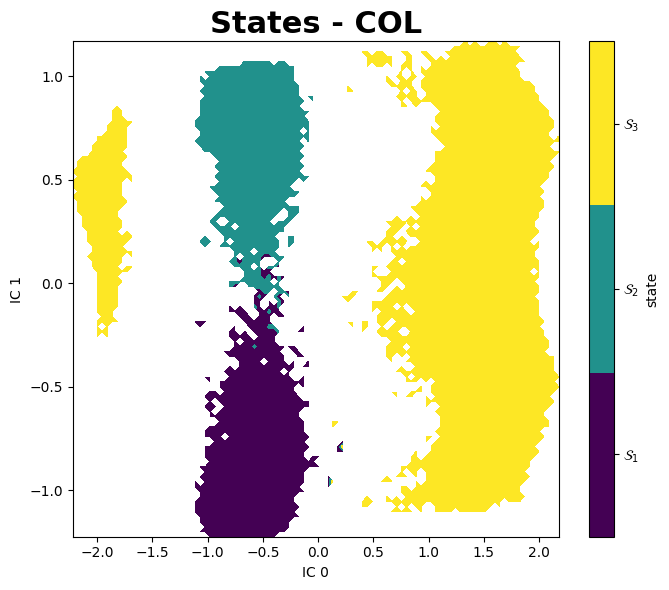
\includegraphics[width=\linewidth]{Images/States_COL_7000K.png}
  \caption{MR-Col}
  \label{MC_states_MR-col}
\end{subfigure}\hfill % <-- "\hfill"
\begin{subfigure}{.45\linewidth}
  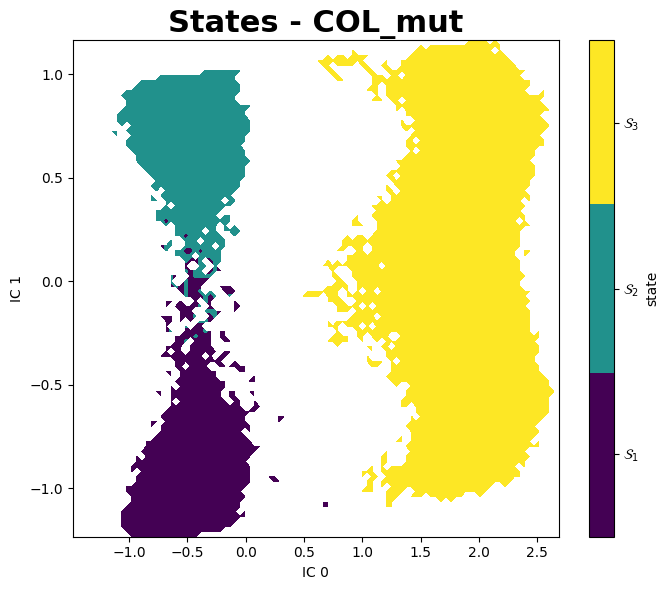
\includegraphics[width=\linewidth]{Images/States_COL_mut_7000K.png}
  \caption{MR$_{mut}$-Col}
  \label{MC_states_MR-col_mut}
\end{subfigure}

\medskip % create some *vertical* separation between the graphs
\begin{subfigure}{.45\linewidth}
  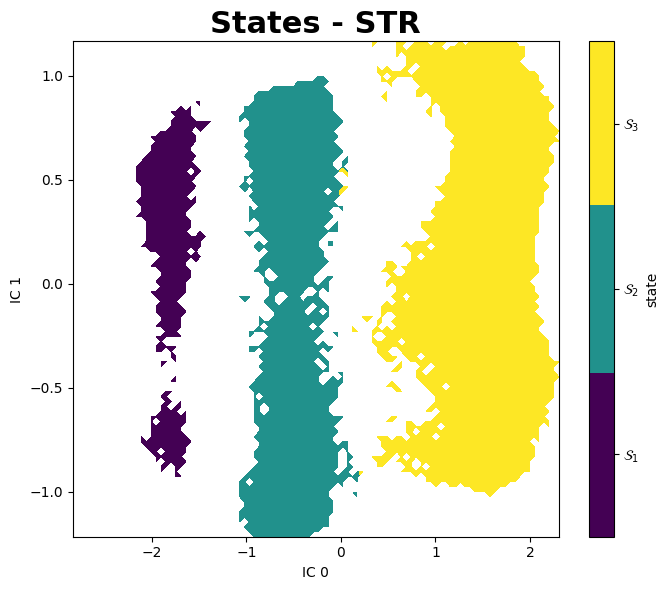
\includegraphics[width=\linewidth]{Images/States_STR_7000K.png}
  \caption{MR-Str}
  \label{MC_states_MR-str}
\end{subfigure}\hfill % <-- "\hfill"
\begin{subfigure}{.45\linewidth}
  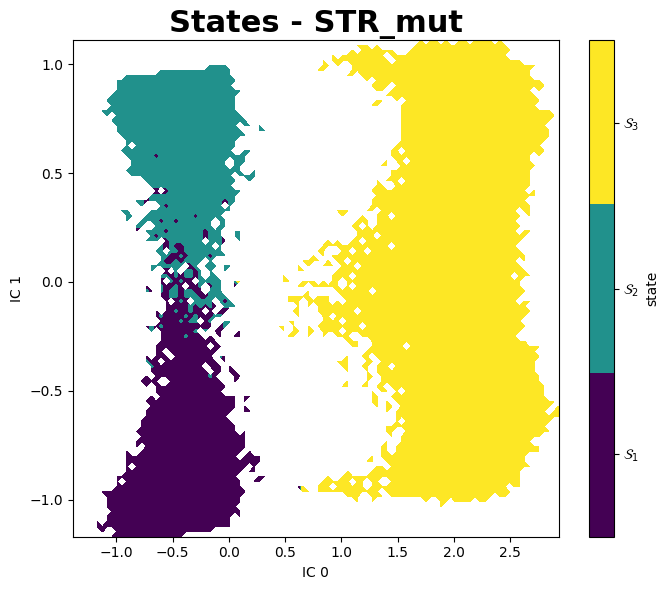
\includegraphics[width=\linewidth]{Images/States_STR_mut_7000K.png}
  \caption{MR$_{mut}$-Str}
  \label{MC_states_MR-str_mut}
\end{subfigure}

\caption{States found with PyEMMA using MC simulations at 7000 K. The first, violet color, represents the flipped state; the second state, green color, represents the bound state; and the third state, color yellow, is the unbinding state for all systems except for MR-STR where PyEMMA could not split the flipped and bound states. }
\label{fig:all-states}
\end{figure}

%\begin{figure}[htbp]
% \centering
% \subcaptionbox{States found for the MR-Aldo system using PyEMMA. The third state (yellow) represents an unbindg macrostate with two microstates: two unbinding pathways that are separated by the first (violet) and second (indigo) state; the first and second states represent the in pocket and flipped microstates, respectively, and both are a binding macrostate.\label{MC_states_MR-as4}}{%
%   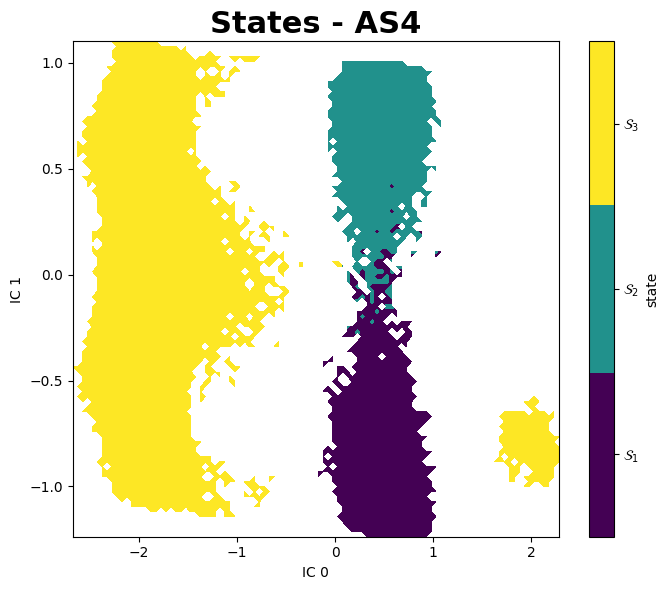
\includegraphics[width=0.9\linewidth]{Images/States_AS4_7000K.png}%
%   }\par\medskip
% \subcaptionbox{States found for the MR-Aldo$_{mut}$ system using PyEMMA. Although the states are the same as in top Figure \ref{MC_states_MR-as4}, the unbinding states of the right disperse and form two microstates.\label{MC_states_MR-as4_mut}}{%
%   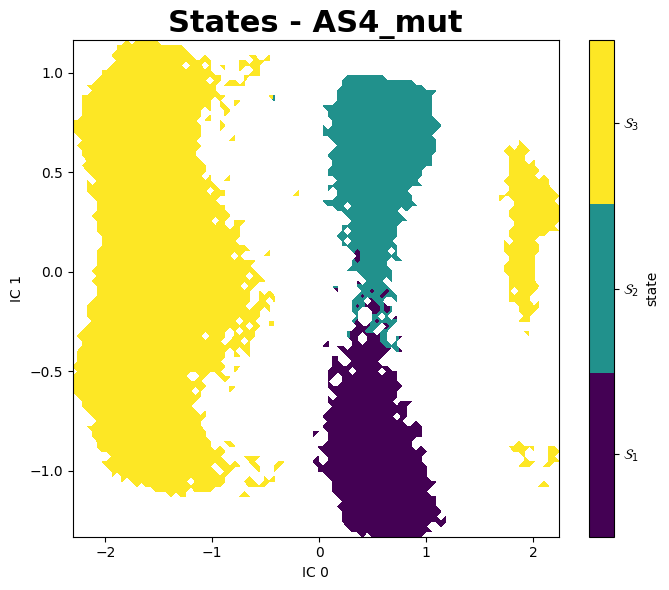
\includegraphics[width=0.9\linewidth]{Images/States_AS4_mut_7000K.png}%
%   }\par\medskip        
% \caption{States found in the MR-MR$_{S810L}$-Aldo system using PyEMMA. For the other systems (Col and Str) the mutation remove the small unbinding state, as can be seen in the Figure \ref{fig:all-states}.
% %this can be seen in the extensive results web page \href{https://saguileran.github.io/MD-SCPI/results/}{MD-SCPI/results/}.
% }
% \label{States_as4}
% \end{figure}




\begin{figure}[htbp]
\centering
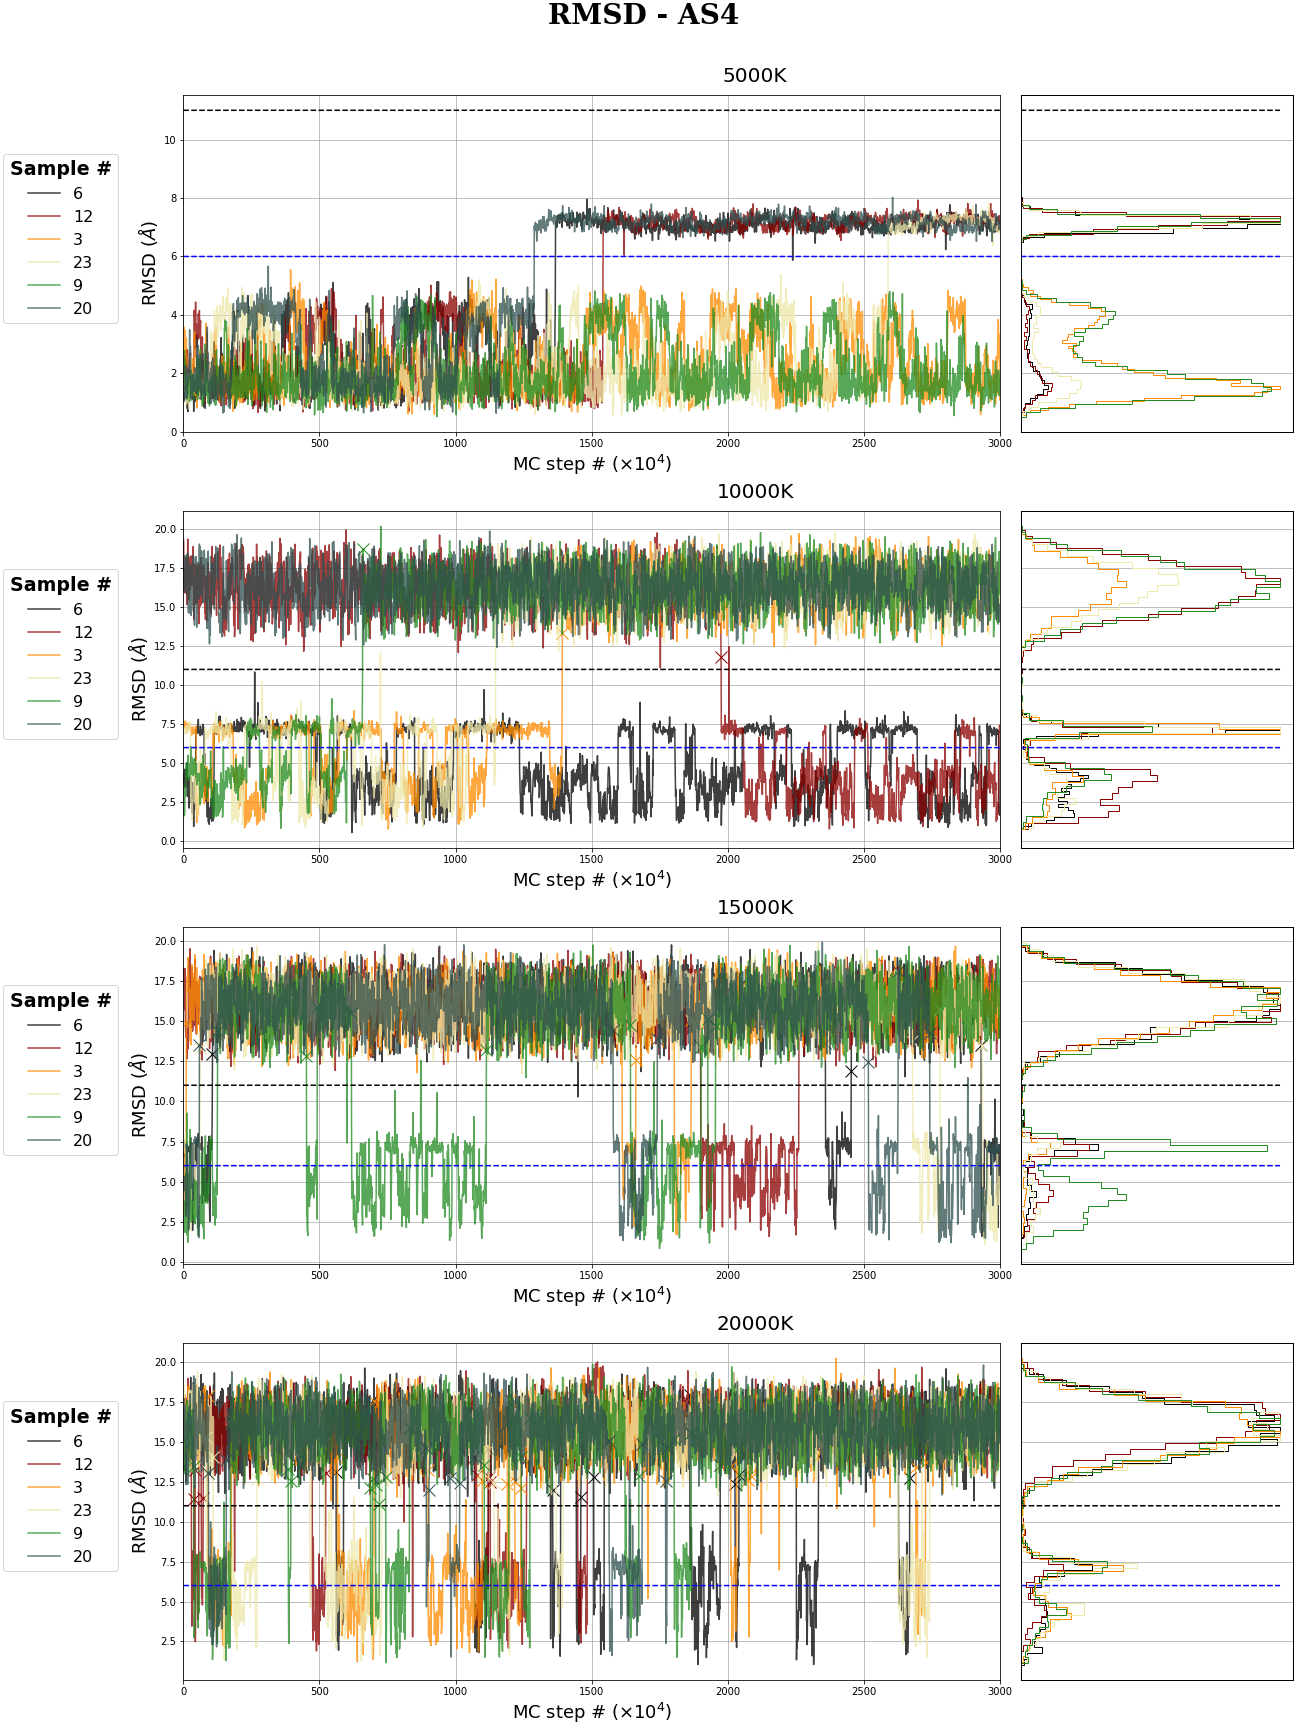
\includegraphics[width=0.95\linewidth]{Images/MC_RMSD_MR-AS4_high.png}
\caption{RMSD as function of LiBELa steps for the MR-Aldo system.}
\label{MC_RMSD_steps}
\end{figure}



\begin{figure*}
\centering
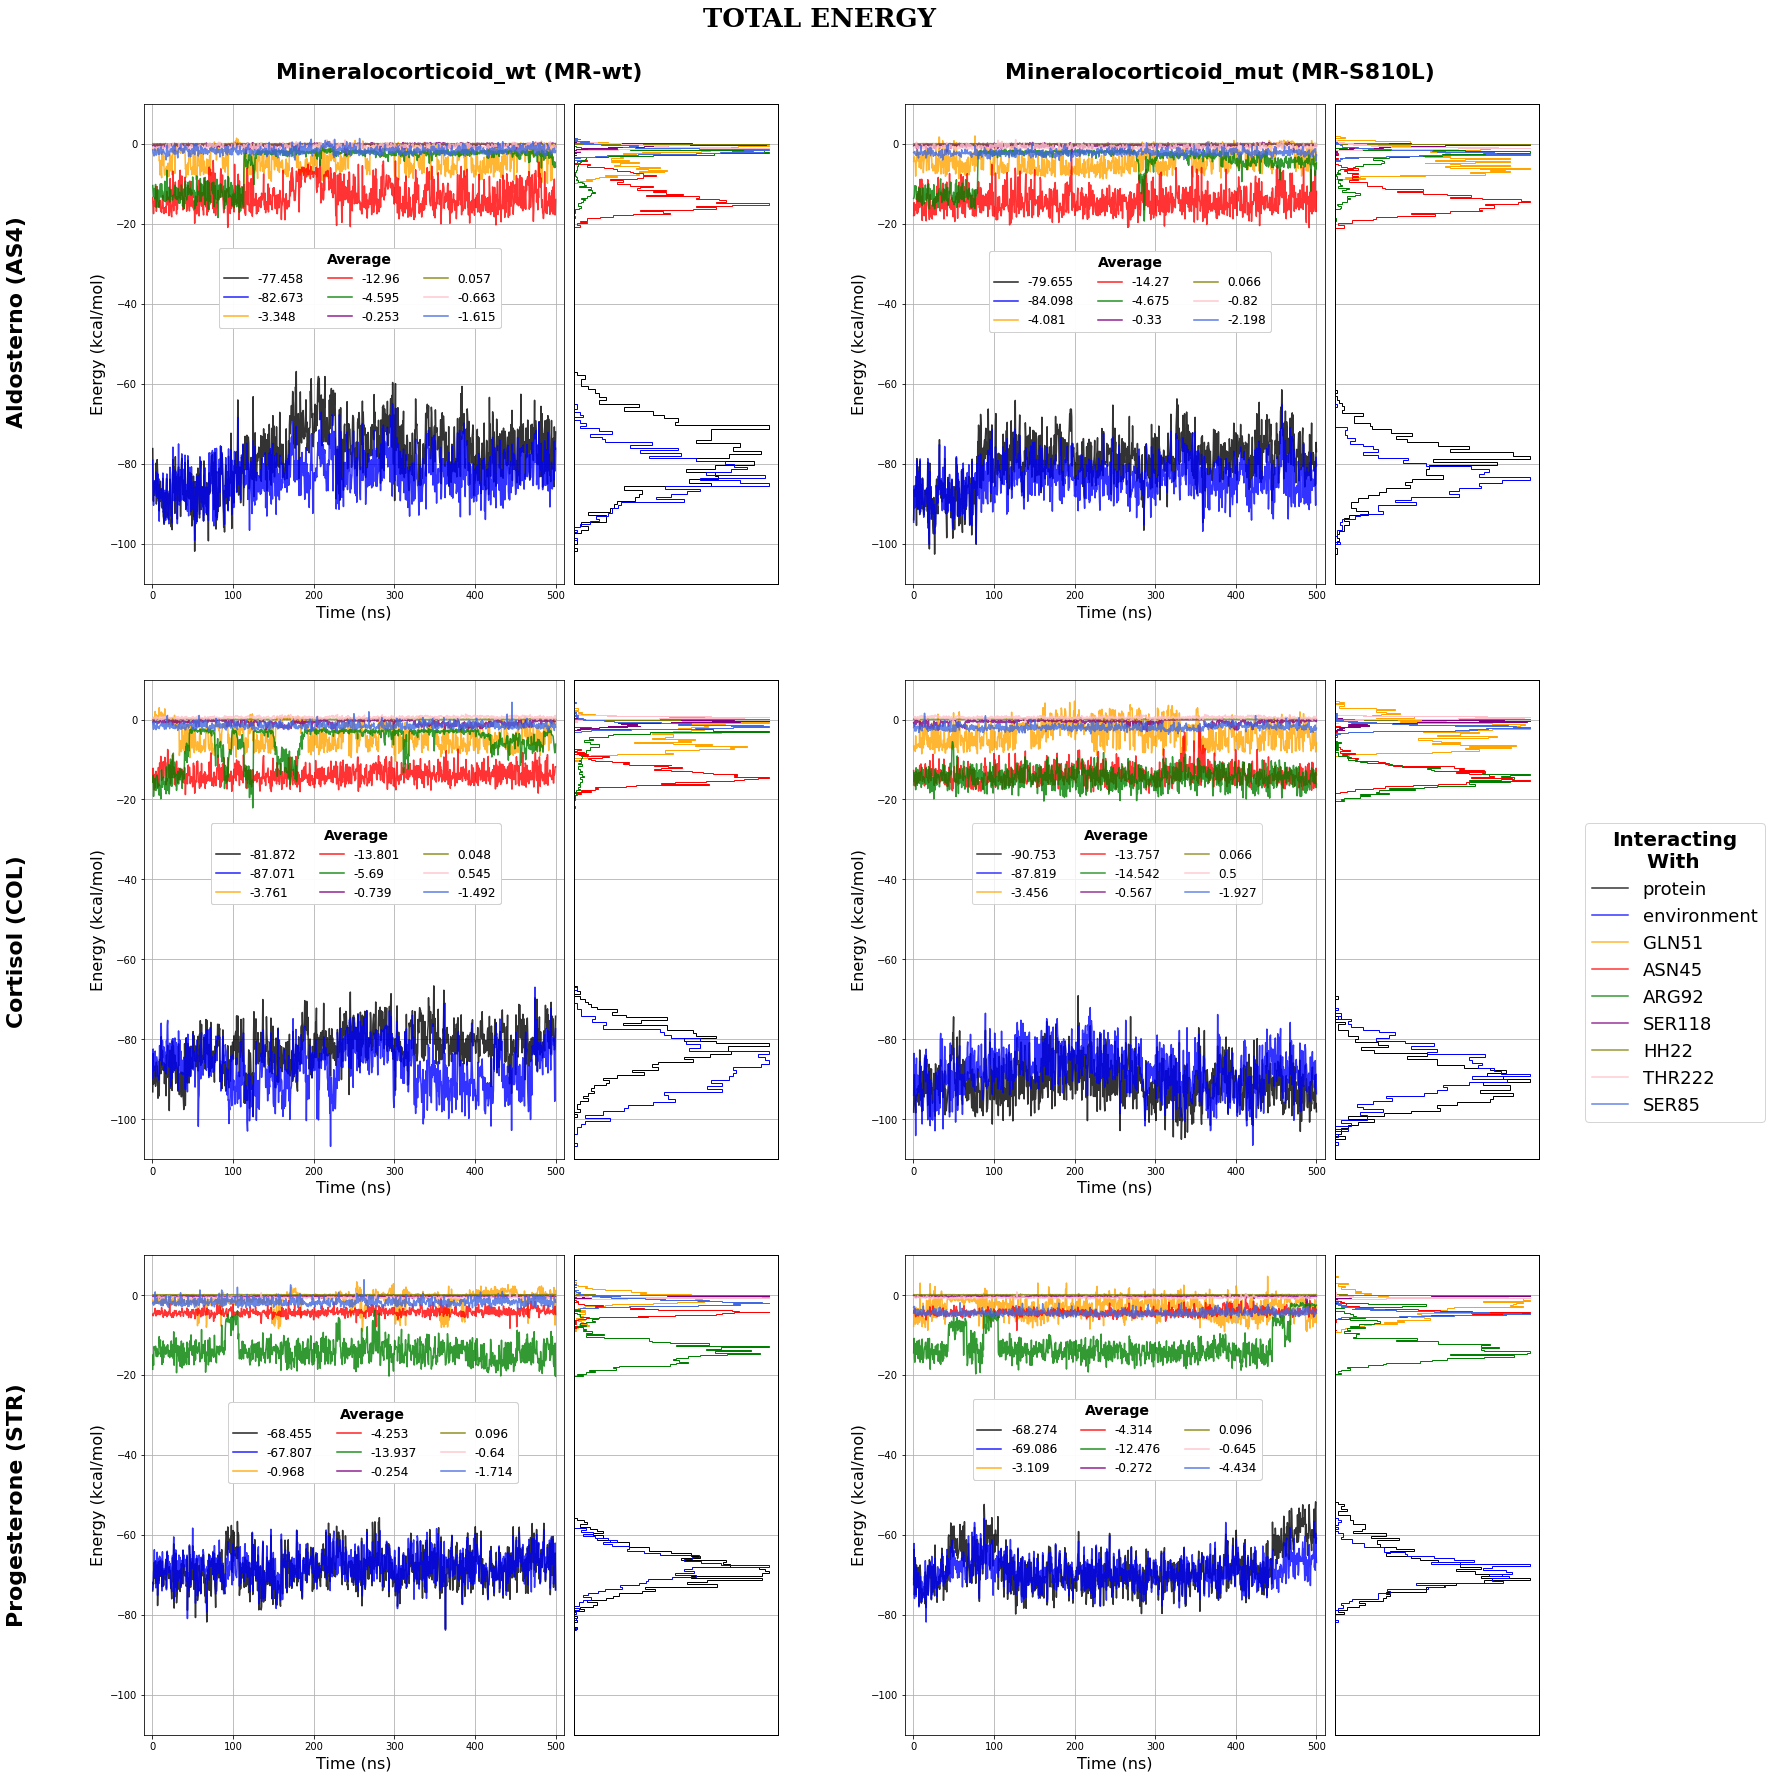
\includegraphics[width=0.99\linewidth]{Images/Energies.png}
\caption{Energies as a function of the MD steps, time, of all systems.}
\label{MD_energies}
\end{figure*}


}

% Lorem ipsum dolor sit amet, consectetur adipiscing elit, sed do eiusmod tempor incididunt ut labore et dolore magna aliqua. Lorem ipsum dolor sit amet, consectetur adipiscing elit, sed do eiusmod tempor incididunt ut labore et dolore magna aliqua. Lorem ipsum dolor sit amet, consectetur adipiscing elit, sed do eiusmod tempor incididunt ut labore et dolore magna aliqua. 


\printendnotes
\clearpage
\onecolumn{
%\bibliographystyle{}
\printbibliography
\nocite{*}
}

\end{document}